\chapter{ROSDashboard: A Visual Debugging System for ROS}
\label{rosdashboard}

[should the chapter be renamed to "prototype" or "prototypical implementation"?]

Write about rosdashboard (overview).

rosdashboard is a prototypical implementation of the system presented in Chapter~\ref{visual_debugging_system} for the ROS middleware / framework. ROS was chosen as middleware because the simple publish/subscribe mechanism allowed to connect to topics transparently without the other party explicitly knowing about the visualization tool.

[Not sure if this is possible in other frameworks, if not it could be stated that more work is needed for those frameworks in order to make communication transparent. In general I can argue that ROS fits the requierements best, the system design was not intended to fit every framework but was developed without compromises current systems might have]

[I'm not sure how to write this chapter: can I have a section "why ROS?", "how the requirements are met?", ...?] ---> this should be written in the introduction for this chapter: ROS was used because it has many users, an easily accesible communication structure, a tool landscape (?) where such a tool would fit in well (recent surge of graphical tools like rxdeveloper, rqt, other dashboards).

\parbox{.8\linewidth}{
[from icra paper, needs some changes]

ROSDashboard, the tool presented in this work, aims to support the developer during debugging by visualizing data in a graphic way and thus eliminating the cognitive effort needed to parse and interpret text based logging messages. While most of the currently available visualization tools in robotics focus on spatial data to help understand the robot and the environment in which it runs \cite{Collett2010, Quigley2009}, rendering of abstract data is still uncommon. ROSDashboard provides a dashboard interface to robot developers, which they can populate with graphical widgets to visualize all kinds of data from the robot. The dashboard can be customized to display widgets according to the current robot hardware and development stage. It can be used to visualize data during debugging as well as monitor data during the normal execution of the robot. This means ROSDashboard is a tool that a) can be adapted to many different use cases and b) allows the developer to choose the widgets he or she thinks represent the data best, according to their mental model and the meaning of the data. The tool is based on ROS (Robot Operating System) which abstracts from specific robot hardware and takes care of inter process communication \cite{Quigley2009}.
}

%%%%% Robot Operating System ROS %%%%%%
\section{Robot Operating System (ROS)}
The Robot Operating System (ROS) is an Open Source framework for complex robotic systems. The first work on ROS was done as part of the STanford Artificial Intelligence Robot (STAIR) in 2007 \cite{Quigley2007}. The original software library was called \emph{Switchyard} and had been developed at Stanford. Later the library was refined and generalized to also suit the requirements of the Personal Robot Program at Willow Garage\footnote{www.willowgarage.com} \cite{Quigley2009}. The resulting general framework has been released as Open Source \cite{Quigley2009} and this section gives a short overview over the most important principles in ROS.

\begin{figure}[ht]
\centering
\subfigure[Stanford's STAIR]{
	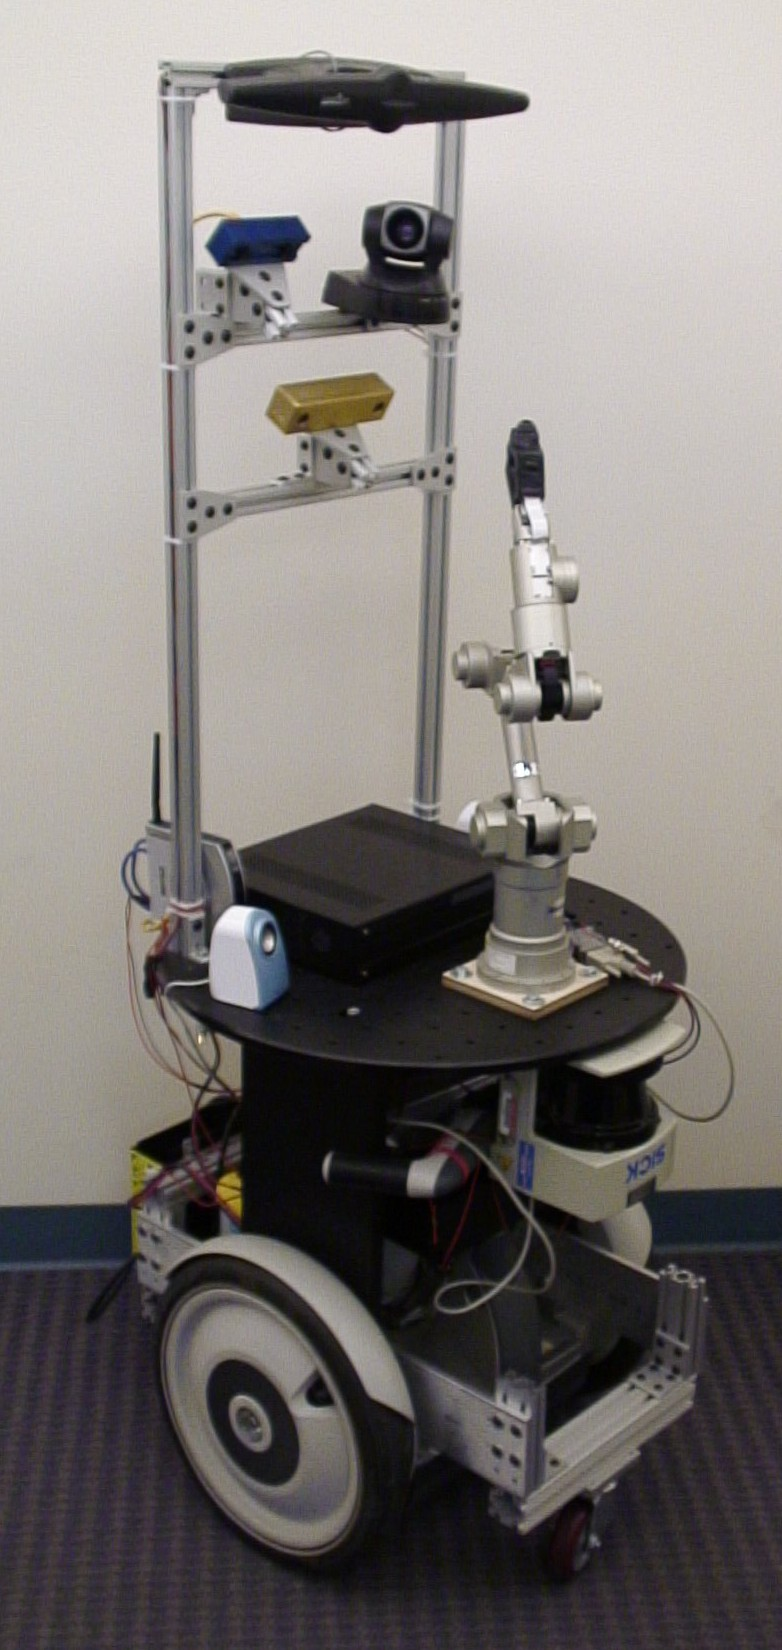
\includegraphics[height=8cm]{img/stair}
}
\subfigure[Willow Garage's PR2]{
	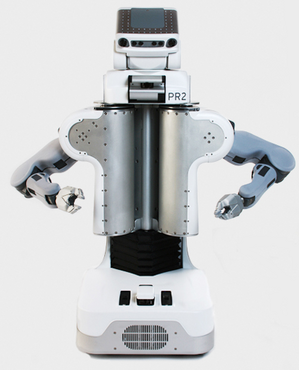
\includegraphics[height=8cm]{img/pr2}
}
\end{figure}

ROS has grown significantly in the last years, it has an active community backing the project and supports many of the currently available robots \cite{Foote2012}. It was developed to abstract from the hardware of the robot and make it easier to create modular robot software, which can run on different robots and on different machines. The modular approach makes development easier, because the work can be divided amongst different developers or development teams. This also allows the developer to change only small parts of a complex system, without the need to build and re-deploy the whole system.
The modules in ROS are called \emph{nodes} and several nodes executed together are called a \emph{stack}. ROS \emph{packages} bundle nodes and stacks and are used to make software modules available to other developers. Everyone can create their own package which can be indexed by ROS so that their software modules can be found, downloaded and used by other developers. There exist many packages, nodes and stacks with implementations of algorithms for some of the most common problems in robotics (e.g. navigation, localization, joint movement, etc.) and they can easily be (re-)used.

The communication between ROS nodes is either asynchronous through a publish/subscribe mechanism or synchronous through services. Nodes can send messages by publishing a message on a topic and receive messages by subscribing to that topic. This mechanism is flexible and decouples the sender from the receiver. A publisher node does not need to know if there are other nodes listening and vice versa. For synchronous communication and guaranteed delivery of messages, services can be invoked. The routing for publish/subscribe messages is established during runtime through the ROS core. The communication between nodes is one of the main sources for debugging data when debugging a ROS application. The same communication framework is also used for the logging mechanism in ROS, which publishes messages to the special purpose topic \emph{/rosout}.

\todo{Overview over this section}

\todo{explain why ros was chosen?}

\todo{list some tools and recent projects that have influenced the tool. For example the rxdeveloper tool and the survey in Muellers2012, RQT and other dashboards recently developed. Highly related to the choice of making a tool for ros.}

\subsection{ROS Publish/Subscribe Mechanism}
\todo{explain the pubsub mechanism in detail? reference here from the system design section which mentiones pub/sub}

\subsection{Related ROS Tools}

\subsubsection{rxplot, rxconsole, rxbag?}
\todo{decide whether to keep this subsection or not}
rxplot is a graphical tool which can plot values from topics on a Cartesian coordinate system. The tool takes data from a published ROS topic and prints it on a time graph. The tool can be configured to visualize several graphs in one go, which makes it easy to compare values and data streams.

[rxplot screenshot, there is not much more to say]

\subsubsection{RQT - ROS GUI}
--> remove from debugging section, not related to debugging. can be introduced in rosdashboard when reasons for the choice of ros are presented (rosdashboard integrates well with other tools in the ros environment and recently many graphical tools were developed)

\subsubsection{rxDeveloper}
[\textbf{outline, results of the survey, importance for this work}]
\cite{Muellers2012}

[Not really debugging, this might go somewhere else? Maybe not a full subsecion but only a couple of sentences that summarize the results and why it is important for this work]

%%%%% Implementation Details %%%%%%
\section{Implementation Details}

\subsection{Visualization Widgets}
\todo{List the currently available visualizations, explain how to add new ones --> show that new widgets can be easily added}

\subsection{Topic Introspection}

\begin{figure}[thpb]
  \centering
  \framebox{
    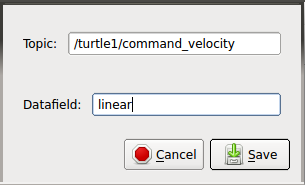
\includegraphics[scale=0.8]{img/topic_setup.png}
  }  
  \caption{Screenshot of the topic setup dialog. [re-do screenshot with rosdashboard in background]}
  \label{topic setup screenshot}
\end{figure}

ROS topics were originally not designed and developed as something the user or developer chooses graphically: They are usually created, configured and used in the source code. ROSDashboard exposes the topic setup in a graphical user interface every time a new widget is added to the dashboard. To make this as easy as possible and without much overhead, a technical solution was chosen to reduce the number of fields to be set during the topic subscription setup. Normally you have to select a topic name and a message data type. The data type can be one of the standard message types like Float, Integer, String and Boolean or a more complex message type which contains more information in a structured message. To access one data element of a message the ``datafield'' field was introduced in the graphical interface. Figure~\ref{topic setup screenshot} shows an exemplary topic setup configuration to access the linear velocity of the \emph{/turtlesim/Velocity} message published to the topic \emph{/turtle1/command\_velocity}. Using Python's duck typing and the \emph{rostopic} module it was possible to avoid the complexity of dynamically binding message type classes during runtime and detect the message type automatically. If a topic is not yet published and thus the message type of this topic is not defined yet, the method call to \emph{rostopic} will block until the message type becomes available. To avoid blocking of the user interface a listener thread was implemented to wait until the message type for a topic becomes available (see Figure~\ref{topic subscription}). Avoiding to manually ask the user for a message type makes the configuration of widgets easier and faster for the user, it also keeps the implementation significantly simpler, because no dynamic binding of message type classes during runtime is needed.

\begin{figure}[thpb]
  \centering
  \framebox{
    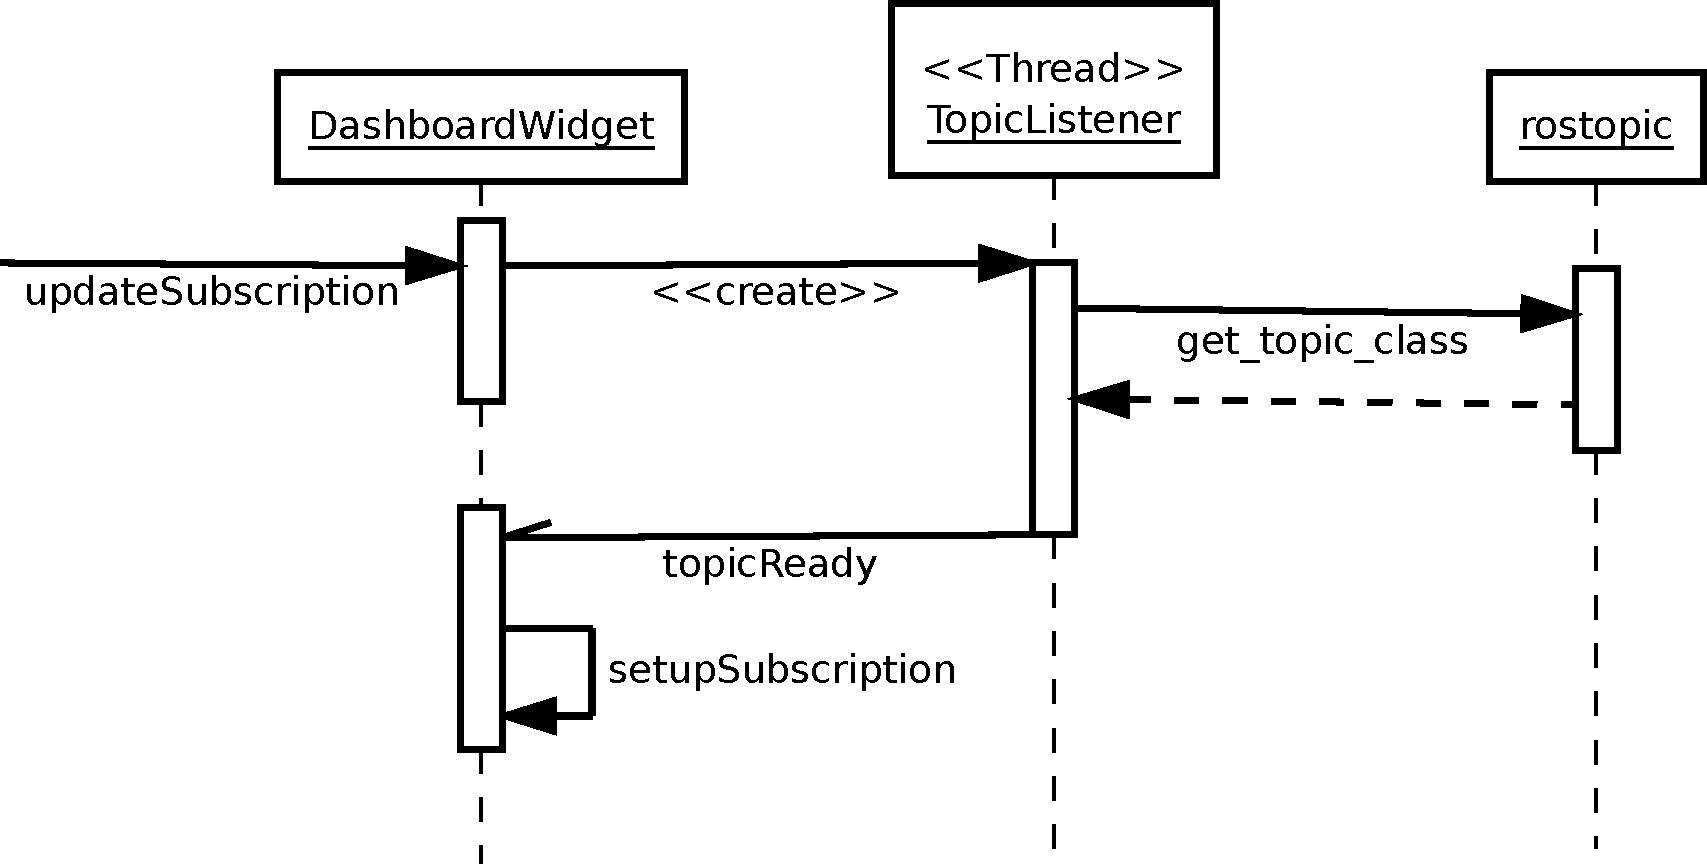
\includegraphics[scale=0.4]{diagrams/topic_subscription.pdf}
  }  
  \caption{Exemplary flow of events for asynchronous topic subscription setup.}
  \label{topic subscription}
\end{figure}

\subsection{User Interface}
[write about the user interface to configure widgets and the feature to delete widgets from the dashboard through drag and drop. should this be in the design?]

\subsection{Plugins}
Reference to the plugin framework section in Chapter~\ref{visual_debugging_system} and that such a system was not yet implemented in ROSDashboard [can I say: due to the time constraints of this work?], but the necessary measures have been taken to allow this in the future. Show some details about an example widget and what methods it overwrites.

\subsection{API}
\begin{lstlisting}[float,frame=single,caption={ROSDashboard API methods.},label=api_calls,language=Python]
# log arbitrary data,
# try to find the data type with introspection
api.log(tag, data)

# log string message
api.logstring(tag, msg)

# log integer value
api.logint(tag, value, msg_type=Int32)

# log float value
api.logfloat(tag, value, msg_type=Float32)

# log complex data with datatype
api.logdata(tag, data, msg_type)
\end{lstlisting}

The current ROS logging framework publishes the log messages on the special purpose topic \emph{/rosout}, but converts everything to a String before the transmission. Since those logging messages are text based, valuable information about the type of the data is lost. To use the data for visualization, the type information must be kept. Thus a set of convenience methods were exposed in the ROSDashboard API (Listing~\ref{api_calls}) to provide a simple interface to publish data for the visualization. The interface is similar to the logging API exposed in the ROS client libraries and basically wraps the ROS specific methods to publish data on a topic. Listing~\ref{api_implementation} shows the simple implementation of the \verb+logint+ API method.

\begin{lstlisting}[float,frame=single,caption={Implemented logint API method.},label=api_implementation,language=Python]
def logint(tag, value, msg_type=std_msgs.msg.Int32):
    """
    publishes a integer value to the /rosdashboard/<tag> topic
    Be careful to use only valid tags, ROS does not allow
    dashes and dots in the topic name.
    
    The default integer message type is std_msg.msg.Int32
    """
    pub = rospy.Publisher('/rosdashboard/' + tag, msg_type)
    pub.publish(msg_type(value))
\end{lstlisting}

The API methods shown in Listing~\ref{api_calls} can be used like logging statements to emit data for visualization. The \verb+TAG+ parameter is used to identify the data when the visualization widgets are set up. Internally the data is published as a message on a ROS topic. The topic name consist of the ROSDashboard specific prefix \emph{/rosdashboard/} and the tag given as parameter. Listing~\ref{exapmle_api_call} shows an example use of the API to publish a integer value with the tag "proximity". The value "7" will be published on the ROS topic \emph{/rosdashboard/proximity} and can be visualized with a widget in ROSDashboard that points to the respective topic name and accesses the "data" datafield of the message.

\begin{lstlisting}[float,frame=single,caption={Example API usage.},label=example_api_call,language=Python]
import rosdashboard

rosdashboard.logint('proximity', 17)
\end{lstlisting}

Although this solution proved to be a useful way to expose data during debugging, it might not be feasible for a bigger project because it introduces a new dependency to ROSDashboard. Since the API is only a set of convenience methods that publish data on ROS topics, data can also be published using the same ROS methods the API uses directly in the target application. Other possible solutions will be discussed as future work in Chaper~\ref{future_work}.
